\chapter{METRICS FOR EVALUATION}

\section{Time to trigger the vehicle prototype}

Since the prototype is linked to the airbag unit, we need to evaluate the time taken for deployment of the airbag itself. Therefore, we consider the various values for \textbf{maximum decelaration} and the time taken for the airbag to deploy for each value. An optimal outcome would be taking less time to deploy for higher values of maximum decelaration.

Formula for decelaration

\[ (u - v) / t \]

where \\
\textit{u} - Initial velocity \\
\textit{v} - Final velocity \\
\textit{t} - Difference in time
		

\begin{figure}[h!]
	\centering
	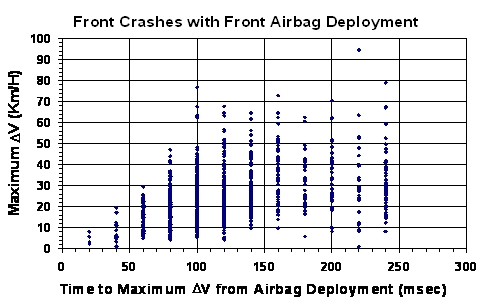
\includegraphics[scale=1]{param1}
	\caption{Time to trigger}
	\label{fig:param1}
\end{figure}

\hfill
\pagebreak
\section{Report latency time}

One of the main keypoints of this project is to reduce the latency in reporting accidents. As such, we present a comparison of various methods of reporting. MERS 999 \cite{aalds} is a response system used in some countries. It is faster when compared to traditional technique, but still suffers \textbf{latency} due to the initial \textbf{verbal communication} involved. Our method eliminates need of verbal communication by providing all the information in the form of easily understandable text, which can also be parsed by machines. Our system was tested based on 20 iterations and the average time taken is 40\% faster than AALDS \cite{aalds}. This indicates a significant time improvement, which could possibly increase time efficiency of emergency services by the authorities.

\hfill

\newcolumntype{Y}{>{\centering\arraybackslash}X}
\renewcommand{\arraystretch}{2}

\begin{tabularx}{\textwidth}{|*{4}{Y|}}
	\hline
	\multirow{2}{*}{Factors} &\multicolumn{3}{c|}{Average Time Taken (sec)}\\
	\cline{2-4}
    &MERS 999	&AALDS	&AVAR\\
    \hline
    Accident Reporting	&50	&20	&10\\
    \hline
	Assess call &112.5	&0.0458	&N/A\\
	\hline
	Notification &N/A &N/A &3.5\\
    \hline
    Total     &162.5 &20.0458	&13.5\\
    \hline
%    \caption{Comparison between methods}
\end{tabularx}

\hfill

\section{Reporting false alarms}

Due to unforeseen circumstances, the airbag might be triggered when not needed in case of minor bumps. In such cases, the user is provided with an option to issue a false alarm notice from his smartphone application. There is a possibility that the user might not use this feature but rather let the report be generated. This may seem harmless, but huge amounts of false positives will only act as noise and may even hinder the reporting of true positives. As such a survey conducted shows \cite{data} that almost 28\% of the respondents wouldn't use the feature. The project should aim to reduce this value by creating an effective way to report false alarms.

\begin{figure}[h!]
	\centering
	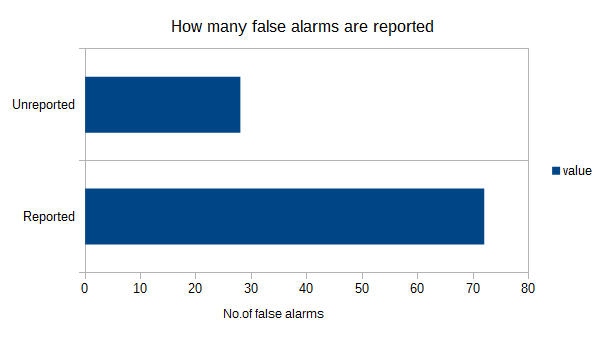
\includegraphics[scale=1]{param3}
	\caption{Reporting false alarms}
	\label{fig:param3}
\end{figure}
